\subsection{RAG-Based Recommendation Systems}

The core of this thesis will be built around my own system, Rag-Poison-Lab \cite{ragpoisonlab_repo}, that englobes all possible fails and risky behavior an actor could affect rankings with from the retrieval to ranking to the final output. A user profile is converted to a query, candidates are retrieved from Elasticsearch, and top-$K$ items are ranked for output and trace inspection.

Those are the basic concepts of a retrieval-augmented generation (RAG) system: if retrieval changes, final model behavior also changes \cite{lewis2020rag}. In a reccomender system, Large Language Models (LLMs) also take care of re-ranking, which opens a window for more risks since retrieved text can hurt the ranking \cite{hou2023llmrankers}. To get the complete picture, I made sure that my system allows for both simple deterministic ranking and LLM re-ranking, which will help us see the result we get from both these recommendation methods.

We will use the dataset MovieLens 100K, a benchmarking dataset containing more than 100,000 rating of 9000 movies by almost 1000 users \cite{harper2015movielens}. The dataset is small enough to run on a local environment which is necessary in the context of using local models.

\subsection{Harmful Retrieval Poisoning Threat Model}

The main risk comes from retrieval poisoning. An attacker won't need to affect the model itself, he can simply corrupt the indexed data so the retriever and ranker push the attackers intended result

This risk is in fact very well documented in recommender security research: factorization-based systems \cite{li2016factorizationpoison}, graph-based systems \cite{fang2018graphpoison}, top-$N$ ranking \cite{fang2020influencepoison}, and deep recommendation models \cite{huang2021deeppoison}. Rag system research also report similar issues: poisonned knowledge can affect what the system generates and how it behaves \cite{zou2024poisonedrag,zhang2025corruptrag}. A specific recommender system research focuse on RAG poisonning also shows poisoned retrieval context can manipulate the output \cite{nazary2025poisonrag}.

to get a complete picture we will thus take a look at three type of attacks that are planned to be available in the local codebase: targeted promotion, prompt injection, and untargeted degradation.

\subsection{Rag-Poison-Lab System Workflow}

Rag Poison Lab contains the whole workflow and is made from scratch to cater to our specific use case. It prepares the data, creates the baseline and poisoned files the indexes them on Elasticsearch, shares recommendation and the API routes and traces, and finally keeps artifacts from every run with a specific run ID \cite{ragpoisonlab_repo}. We are eseentially  trying to design 2 flows one where the system is not attacked and one where it is and then compare the results from the run through two indices: \texttt{movies} and \texttt{movies\_poisoned}. 

\begin{figure}[htbp]
  \centering
  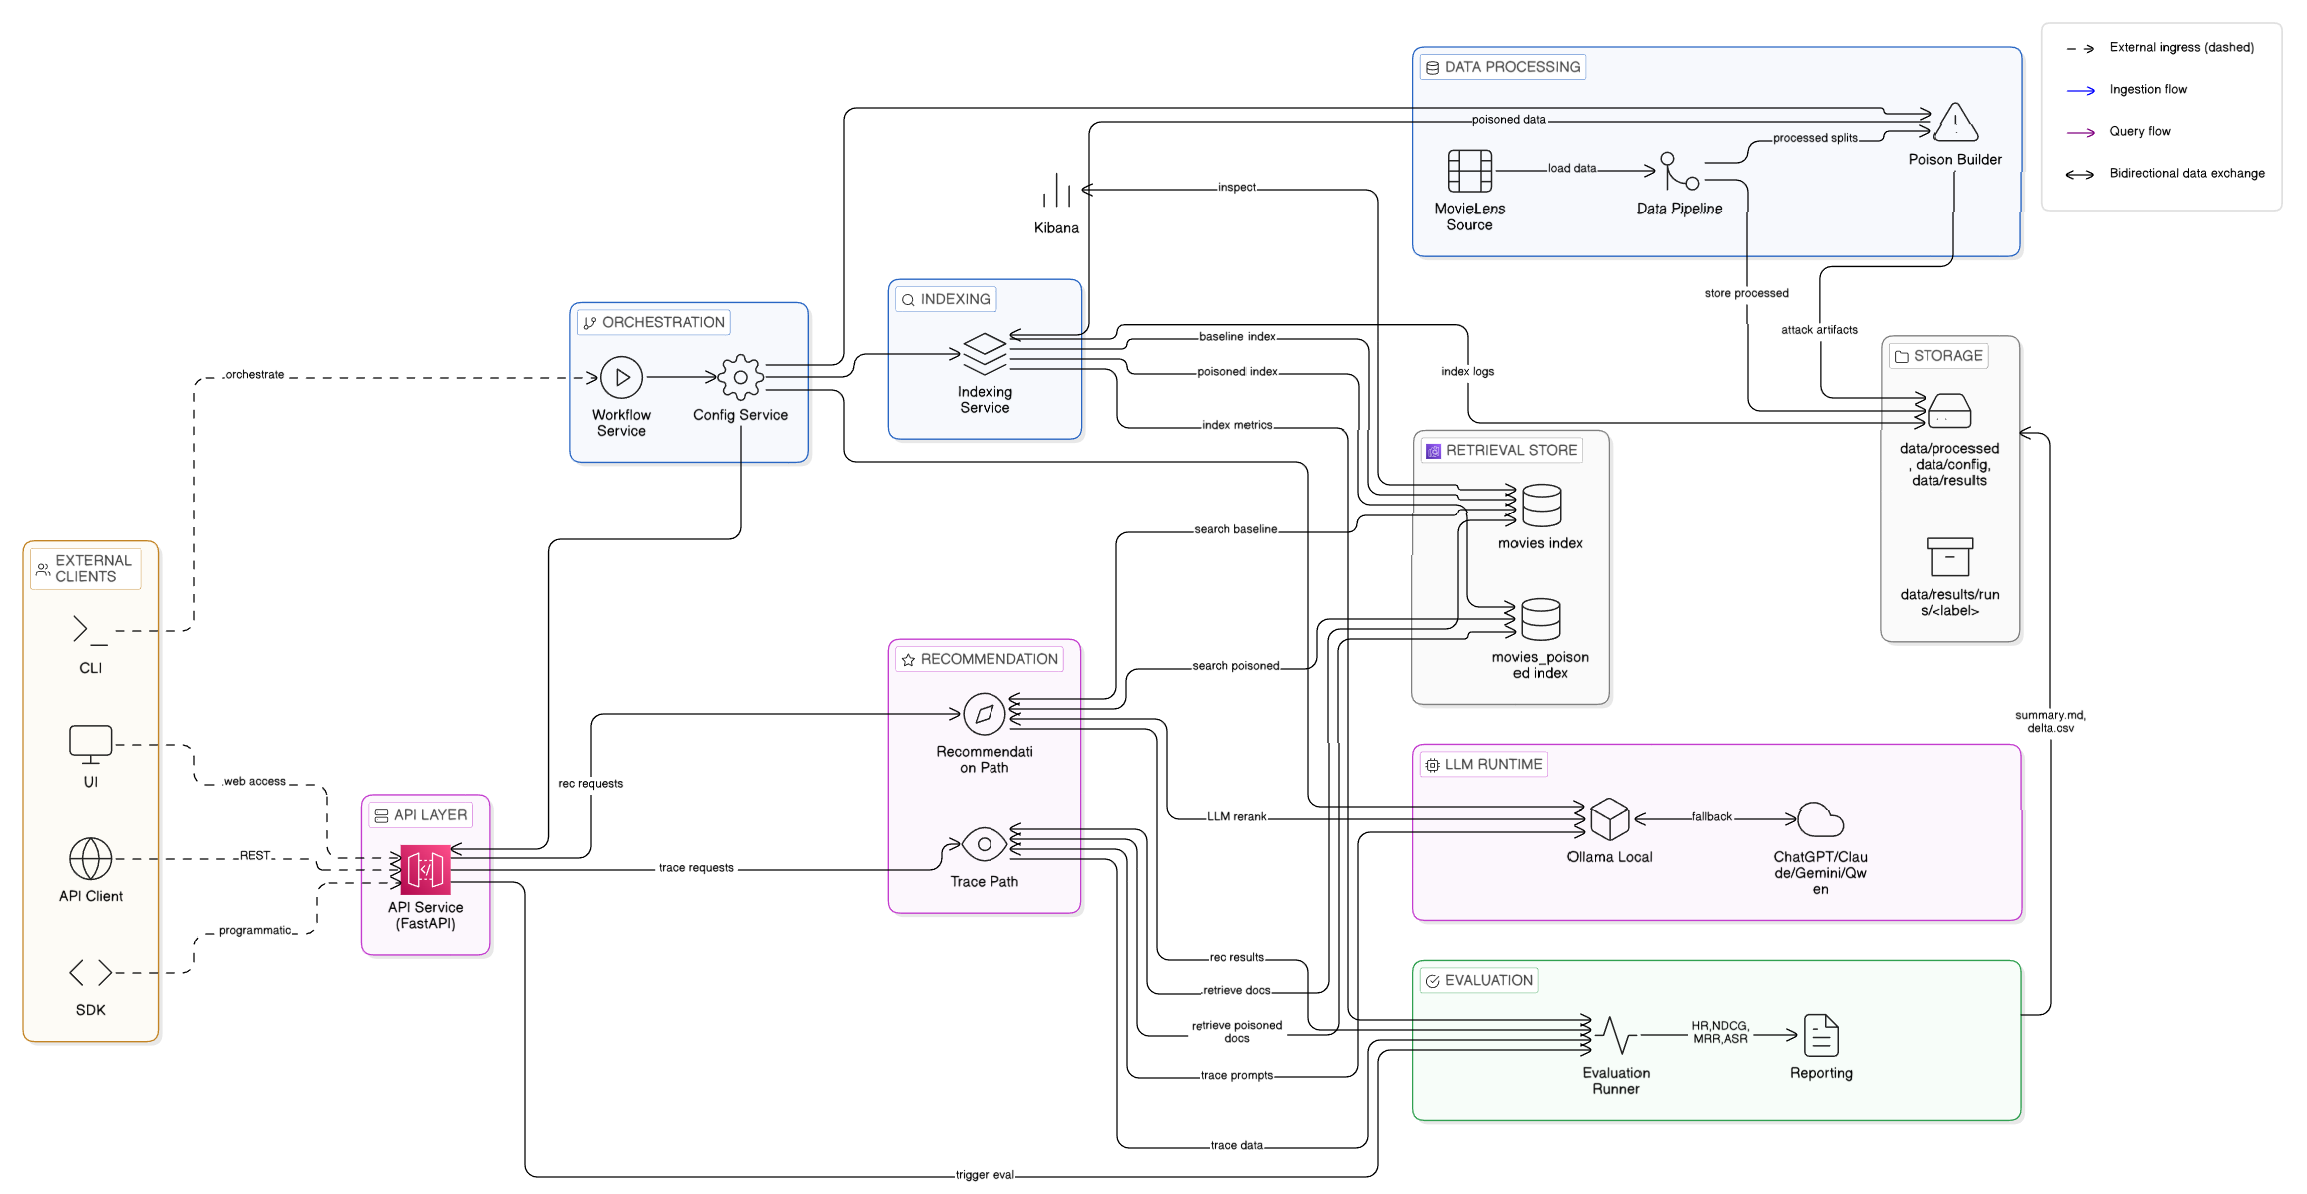
\includegraphics[width=1.0\textwidth]{figures/architecture.png}
  \caption{Planned architecture figure for Rag-Poison-Lab.}
  \label{fig:system-architecture}
\end{figure}

The trace path exposes retrieval query text, retrieved documents, poison markers, and re-ranking internals. This is important for our poisonning evaluation because it shows why the attacks happen and how they work.


\begin{figure}[htbp]
  \centering
  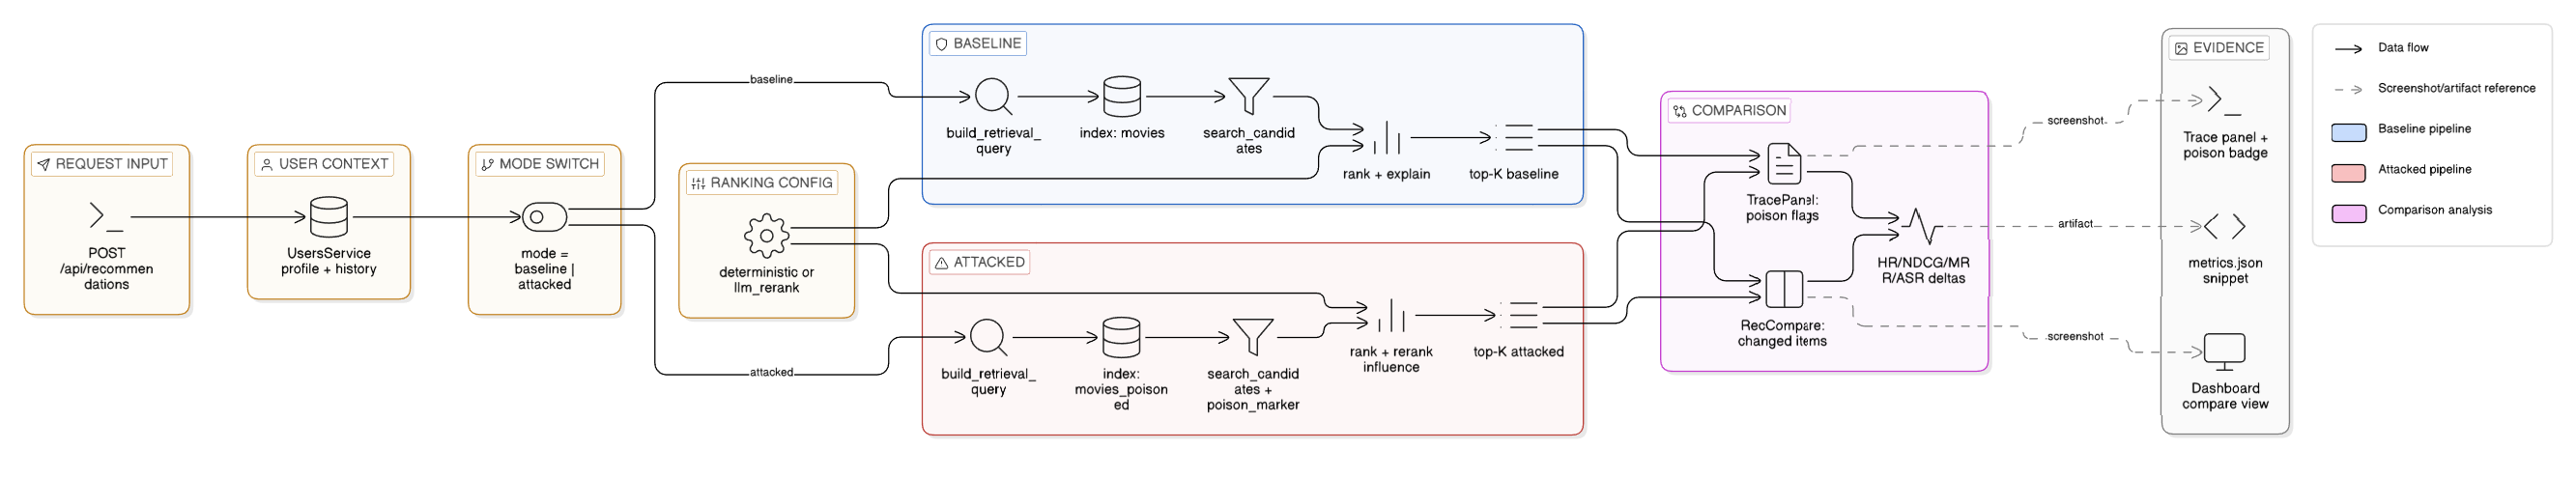
\includegraphics[width=1.0\textwidth]{figures/baseline_vs_attacked_workflow.png}
  \caption{Planned baseline-versus-attacked comparison workflow.}
  \label{fig:baseline-attacked-workflow}
\end{figure}

In short, the project provides a controlled red team lab where the user request is fixed and only retrieval/index mode changes.
